\documentclass[a4paper]{report}

% fonts
\usepackage[T1]{fontenc}
\usepackage{inconsolata}
\usepackage[kerning,spacing]{microtype}
\usepackage[charter]{mathdesign}

% index creation
\usepackage{makeidx}
\makeindex

% miscellaneous packages
\usepackage{xcolor}
\usepackage{hyperref}
\usepackage{verbatim}
\usepackage{siunitx}
\usepackage{todonotes}

% references
\usepackage[backend=biber,sorting=none]{biblatex}
%\bibliography{project.bib}
\addbibresource{project.bib}


% tikz
\usepackage{tikz}
\usetikzlibrary{shapes,backgrounds,decorations.pathreplacing,positioning,fit,shadings}

% algorithms typesetting.
\usepackage{algorithm}
\usepackage{algpseudocode}

\newcommand*\Let[2]{\State #1 $\gets$ #2}

\algblockdefx[REPEAT]
{Repeat}
{EndRepeat}
[1]{\algorithmicrepeat\ #1 \ \algorithmicdo}
{\algorithmicend \ \algorithmicrepeat}


% miscellaneous configurations
\pagestyle{headings}

\hyphenpenalty=100000

% macros

\newcommand{\inputtikz}[1]{\input{tikz_img/#1}}

\newcommand*\BitAnd{\mathrel{\&}}
\newcommand*\BitOr{\mathrel{|}}
\newcommand*\ShiftLeft{\ll}
\newcommand*\ShiftRight{\gg}
\newcommand*\BitNeg{\ensuremath{\mathord{\sim}}}

\begin{document}

\begin{titlepage}
  \centering
  \vspace*{5\baselineskip}
  \huge
  \textsc{Marks Gymnasieskola} \\
  \vspace*{6\baselineskip}
  \Huge
  \bfseries
  How do image file formats work? \\[3\baselineskip]
  \large
  An exploration of the inner workings of image file formats.
  \vfill
  Eric P Arneb�ck \\
  \textbf{\today} \\[2\baselineskip]
\end{titlepage}

\tableofcontents

\listofalgorithms

\setlength{\parskip}{1ex plus 0.5ex minus 0.2ex}
\setlength{\parindent}{0pt}

\part{Preliminaries}

\begin{comment}
  \bibliography{project.bib}
\end{comment}

\chapter{Digital Image}
\label{cha:digital-image}

\section{Color}
\label{sec:color}

\subsection{What is color?}
\label{sec:what-color}

\newcommand{\bluewave}{\ensuremath{\SI{400}{\nano\meter}}}

Color is light. Light on the other hand, is composed of tiny particles
traveling at different wavelengths. \cite{neider93:_openg_progr_guide}
So light is just a wave. Figure \ref{fig:wave} demonstrates what a
wave looks like and what a wavelength measures. Different colors have
different wavelengths. For example: blue, as shown in figure
\ref{fig:wave}, has a wavelength of
\bluewave. \cite{ohlsson99:_digit_bild_kreat} That's $0.00000004$
meters!

\begin{figure}[h!]
  \centering
  \inputtikz{wave.tex}
  \caption{A blue lightwave. $\lambda$ is the letter commonly used to
    represent  wavelength.}
  \label{fig:wave}
\end{figure}

But how do our eyes see these light waves? In our eyes, there are
cells for perceiving three different kinds of wavelengths of light:
red, blue and green. When these cells absorb light, we see color. And
when these cells absorb mixed amounts and/or different amounts of red,
blue and green light, we are able to perceive \textit{all} the other
possible colors.

\subsection{RGB}
\label{sec:rgb}

Color models are ways specifying color numerically \todo{mention
  additive and subtractive color models here}
\cite{fadgi11:color_model}. They are of course very convenient for
computer since they are very good at dealing with numbers. A very
widely used color model for representing color in computer is
\textbf{RGB} \index{RGB}.

\begin{figure}[h]
  \centering
  \inputtikz{rgb.tex}
  \caption{RGB color model}
  \label{fig:rgb}
\end{figure}

The color model is, of course, based on how our eyes perceive color, as
mentioned in section \ref{set:what-color}. Do, however, observe figure
\ref{fig:rgb}. As it can be seen, all the other colors can be achieved
by mixing red, blue and green. Also note that white is achieved by
mixing all of three colors. And black is represented by no light at
all. One last thing: The different values for red, blue and green are
their channels.

\subsection{CMYK}
\label{sec:cmyk}

\subsection{Alpha channel}
\label{sec:alpha_chan}

But there is actually even more to RGB. There is an extended color
model of RGB that's called RGBA \index{RGBA}(it is sometimes also
referred to as ARGB \index{ARGB}). In this model a new channel is
added: the alpha channel \index{alpha channel}. This new channel
represents the opacity of a color. Opacity is simply the opposite of
transparency. Thus, a low transparency means that the color in
question is close to invisible  \cite{porter84_compos_dig_img}.

\section{Color depth}
\label{sec:color-depth}

\newcommand{\rgbtrip}[3]{( \textcolor{red}{#1},\textcolor{green}{#2},\textcolor{blue}{#3})}

But up until now, we have said nothing about how the computer
represents these color model. Let us start with:

\subsection{24-bit color}
\label{sec:24-bit-color}

So each color is just a combination red,blue and green lights. In the
RGB color model these channels are given values. Let us represent
these values as a triple of three numbers, like this:
\rgbtrip{123}{21}{91}.

An 8-bit number has ,as familiar, only $255$ possible values. If we
assign an  8-bit number to each color channel, the color's total size
will be 24-bits. This way of representing color is called 24-bit color
\index{24-bit color}. You can also say that its color depth \index{color
  depth} is 24 bits.

A full red color is represented by the triple \rgbtrip{255}{0}{0}. In
that case, have a guess at what color is represented by
\rgbtrip{255}{0}{255}. If haven't guessed it already, please study
figure \ref{fig:rgb}. As you probably already have guessed, this color
is yellow. And in the same number mixing and matching way, many other
colors can be represented. Like it is represented in color table
\ref{tab:color-examples}

\newcommand{\colorrow}[4]{  \rgbtrip{#1}{#2}{#3} &
  \textcolor[RGB]{#1,#2,#3}{#4} \\ \hline}

\begin{table}[h!]
  \centering
  \begin{tabular}[h!]{|l|l|}
    \hline
    RGB triple & Resulting color \\ \hline
    \colorrow{255}{215}{0}{Gold}
    \colorrow{165}{42}{42}{Brown}
    \colorrow{255}{0}{255}{Purple}
    \colorrow{255}{192}{203}{Pink}
    \colorrow{255}{165}{0}{Orange}
  \end{tabular}
  \caption{Colors}
  \label{tab:color-examples}
\end{table}

But of course, not all colors can be represented using just
24-bit. The number of All possible colors is infinite. But you can
represent an awful not colors with only 24-bits. How many? Well, every
color channel can have $256$ different values. There are $3$
channels. Hence, there are $256^3 = 16777216$ different colors.

\begin{figure}[h!]
  \centering
  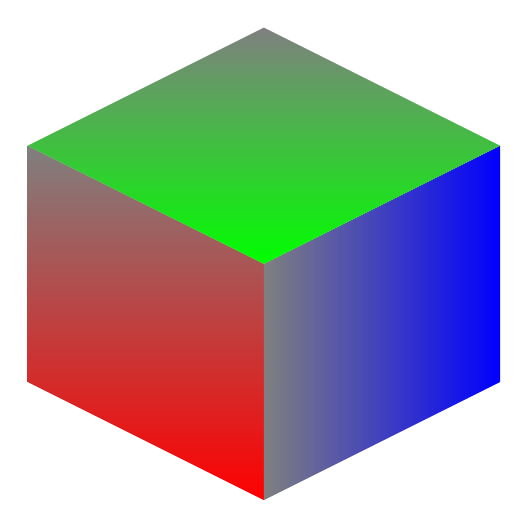
\begin{tikzpicture}
    \shade[yslant=-0.5,bottom color=red]
    (0,0) rectangle +(3,3);

    \shade[yslant=0.5,right color=blue]
    (3,-3) rectangle +(3,3);

    \shade[yslant=0.5,xslant=-1,bottom color=green] (6,3) rectangle +(-3,-3);

  \end{tikzpicture}
  \caption{RGB color cube TODO: Make.}
  \label{fig:color-cube}
\end{figure}

\newcommand{\rgbaquad}[4]{(
  \textcolor{red}{#1},\textcolor{green}{#2},\textcolor{blue}{#3},\textcolor{gray}{#4} )}

Adding alpha channels to this color representation is trivial, just
add a fourth channel. Here is for example the color green halve
transparent: \rgbaquad{0}{0}{255}{125}. The only real difference is
that a color will require 32-bits of storage if an alpha channel is needed.

\subsection{Other colors depths}
\label{sec:other-colors-depths}

\subsection{Indexed Color}
\label{sec:indexed-color}

% 8-bit color 1-bit color, palettes need to be covered.-

\printbibliography[heading=subbibliography]

\begin{comment}
  \bibliography{project.bib}
\end{comment}

\chapter{Compression techniques}
\label{cha:digital-image}

\begin{refsection}

\section{Some terminology}
\label{sec:some-terminology}

Coding a data into another form is often referred to as
\textbf{encoding} \index{encoding}. Converting that encoded data back
into its orginal form is called \textbf{decoding}
\index{decoding}. \todo{Need sources on these two terms.}. In the
circumstanes of compression techniques, encoding is also often
referred to as \textbf{compression} \index{compression}, and decoding as
\textbf{decompression} \index{decompression} or \textbf{uncompression} \index{uncompression}

% http://www.digitizationguidelines.gov/term.php?term=encoder

\section{Bitwise operators}
\label{sec:bitwise-operators}

In this chapter we will start using the bitwise operator. If you
haven't even heard of them, look up them and study them on your own. I
assumed from the beginning of this book that such knowledge should be
obvious to you. We will be using the notation introduced in C to
represent them in pseudocode.

% looks ugly when typeset.
\begin{description}
\item[$\BitNeg$] Bitwise \textit{NOT}
\item[$\BitAnd$] Bitwise \textit{AND}
\item[$\BitOr$] Bitwise \textit{OR}
\item[$\BitXor$] Bitwise \textit{XOR}
\item[$\ShiftLeft$] Left bit shift
\item[$\ShiftRight$] Right bit shift
\end{description}

Notice that we are using $\BitXor$ for typesetting bitwise
\textit{XOR}, rather than the tradtional c notation. This is due to
the fact that we'd otherwise confuse it with logical and, $\AND$.

\section{Pseudocode Functions}
\label{sec:pseudocode}

We will be using several functions in the pseudocode.

\textproc{ReadByte} It is assumed from the beginning of the algorithm that
a file has already been opening for reading. This could be the file
we're trying to compress, uncompress, and many other things. This
function reads a byte from that file.

\textproc{EndOfFileReached} true of the end the file we're reading
from have been reached.

\textproc{WriteByte} At the beginning of every algorithm, we assume
that there is a file opened for output. This function Writes a byte to
that opened file.

We will also a be using custom control structure, repeat:

\begin{algorithm}[h]
  \caption{The repeat control structure.}
  \label{alg:repeat}
  \begin{algorithmic}[1]
    \Repeat{$n$}
      \State $actions...$ \Comment{Repeats $actions...$ $n$ times} %
    \EndRepeat
  \end{algorithmic}
\end{algorithm}

Although we will be dealing in bytes in most of these algorithms, they
could easily by generalized to larger integer types likes
\texttt{long}.

\newcommand{\commentsymbol}{\(\triangleright\)}
\algrenewcommand{\algorithmiccomment}[1]{\hfill\commentsymbol#1}

Comments are signified by the symbol \commentsymbol.

\section{Run Length Encoding}
\label{sec:rle}

\subsection{Naive version}
\label{sec:most-simple-version}

One the most simple compression algorithms is known as Run Length
Encoding \index{Run Length Encoding}(RLE
\index{RLE}). \cite{nagarajan11:_enhan_approac_run_lengt_encod_schem}
The algorithm works like: Sequences of consecutive
data is stored with a data count and a single value rather than the entire
run in packets.

But what does that mean? Let us consider the string

\begin{indentpar}
  WWWWAAAACCCCCCQ
\end{indentpar}

When running the RLE encoding algorithm on this string, it is
compressed like this:

\begin{indentpar}
  4W4A6C1Q
\end{indentpar}

So all the RLE encoding algorithm really do is encode long consequtive
runs of the same value as a count and a single data value. We will call a
sequence of a data count and the data itself a run length
\textit{packet} \index{packet}.

But however, the same thing is also done for single runs, meaning that
the algorithm can potentially explode the size of the original data,
rather than compress it. Consider, for example, the string

\begin{indentpar}
  eric
\end{indentpar}

this will actually get ``compressed'' down to

\begin{indentpar}
  1e1r1i1c
\end{indentpar}

So the size actually doubled for this kind of data! So for very data
with very varying values, like photos and books, this algorithm will
do just horrible. But in data in which the values are not varied much
at all, like that robot logo we showed in the last chapter, even for such a
naive algorithm, it will do quite good.

But this is essentially trivial to implement in code. Let us first
consider the compression algorithm, which is shown in algorithm \ref{alg:rle-enc}

\newcommand{\eof}{\ensuremath{\VoidCall{EndOfFileReached}}}
\newcommand{\neof}{\ensuremath{\NOT \VoidCall{EndOfFileReached}}}

\begin{algorithm}[h]
  \caption{Encoding a file using RLE.}
  \label{alg:rle-enc}
  \begin{algorithmic}[1]

    \Let{$length$}{$1$}
    \Let{$passedFirstCharacter$}{\False}
    \Let{$c_2$}{ \VoidCall{ReadByte}}

    \While{\neof}

      \If{$passedFirstCharacter$}
        \If{$c_2 = c_1 \AND length < 255$}
          \Let{$length$}{$1 + length$}
        \Else
          \State \Call{WriteByte}{$length$}
          \State \Call{WriteByte}{$c_1$}
          \Let{$length$}{$1$}
        \EndIf
      \EndIf

      \Let{$passedFirstCharacter$}{\True} %
      \Let{$c_1$}{$c_2$}
      \Let{$c_2$}{ \VoidCall{Read}}

    \EndWhile

    \If{$passedFirstCharacter$} \Comment{Write the last bytes.}
      \State \Call{WriteByte}{$length$}
      \State \Call{WriteByte}{$c_1$}
    \EndIf
  \end{algorithmic}
\end{algorithm}

The ridiculously simple RLE decoding algorithm is shown in algorithm
\ref{alg:rle-dec}

\begin{algorithm}[h]
  \caption{Decoding a RLE encoded file.}
  \label{alg:rle-dec}
  \begin{algorithmic}[1]

    \While{\neof}
      \Let{$length$}{\VoidCall{ReadByte}}
      \Let{$c$}{\Call{Read}{}}

      \If{\eof}
        \Break
      \EndIf

      \Repeat{$length$}
        \State \Call{WriteByte}{$b$}
      \EndRepeat
    \EndWhile
  \end{algorithmic}
\end{algorithm}

All we're really doing here is reading packet length and the packet
data and then outputting that data length times to a file.

\subsection{Packets version}
\label{sec:packets-version}

But as previously stated,this algorithm just do horrible on data that
is not at all repetitive, like this:

\begin{indentpar}
  ERICARNE
\end{indentpar}

It will get ``compressed'' down to

\begin{indentpar}
  1E1R1I1C1A1R1N1E
\end{indentpar}

Which is double the size. But we needn't forget that algorithm can
do wonders on data that is actually repetitive like for example

\begin{indentpar}
  WWWWWWWWWWWWAAAAAAAAAAAAAAARRRRRRRRRRRR
\end{indentpar}

So, the question is, can we get rid of potentially doubling the size,
yet still being able to greatly compress data such as the
above. Turns out that we can.

We just need to revise out packet format a tiny bit. A byte could be
written as the following bit pattern

\begin{indentpar}
  $00000000$
\end{indentpar}

Now let us reserve the last bit for a flag, and use the rest
for specifying the size.

\begin{indentpar}
  $\overbrace{0}^ \text{Flag bit}\underbrace{0000000}_ \text{Length bits}$
\end{indentpar}

But this last bit won't of course be wasted, it will specify the type
of the packet. If the value of the it is 1, it will be a raw packet,
elsewhise it will be a run length packet. A run-length packet is just
your ordinary packet we used in the naive version. But however, raw
packet means that the data following the firs byte of the packet is
entirely uncompressed and is a sequence of raw bytes. The length of
this sequence, is the value specified by the first seven bytes. And
the length of a run-length packet is also these seven first
bytes. Hence, the new maximum length of a run length packet is the
maximum number of an unsigned 7-bit number, which is $2^7 -1 = 127$.

So we have lost some valuable storage space, but what did we get in
return? Well, now the string

\begin{indentpar}
  ERICARNE
\end{indentpar}

gets compressed down

\begin{indentpar}
  136ERICARNE
\end{indentpar}

(do remember that 136 is a byte of the value 136, and not the sequence
of the number 1,2 and 6)

Which is a huge gain!

But why is the number so huge? Well, that obviously becuase the last
bit flag in a byte has the value $128$. We can toggle that last flag
like this: $136 \BitXor 128 = 8$. And doing that operation we end up with
the value $8$, which is the length of the raw packet.


And while \textit{not} exploding the size of certain kinds of data,
this algorithms can also reap all the benefits the old naive version
of the algorithm had. So the string

\begin{indentpar}
  WWWWAAAACCCCCC
\end{indentpar}

still gets compressed down to

\begin{indentpar}
  4W4A6C
\end{indentpar}

And all of this in exchange for just one bit!

As an exercise for the reader, examine the following compression and
validate its correctness:

\begin{indentpar}
  EEEEEEERIC
\end{indentpar}

to

\begin{indentpar}
  7E131RIC
\end{indentpar}

Now let's so how we can implement these algorithms. It will be a bit
harder than the naive version, but we will soon find that it is not very
difficult at all!

This algorithm is actually the one used to compress color data in the
TGA image format \cite{91:_truev_tga_file_format_specif}.

\subsection{Implementation}
\label{sec:implementation}

\subsubsection{Writing the packets}
\label{sec:writing-packets}

Let us first consider how to write a raw packet. Consider the function
\textproc{writeRawPacket}(algorithm \ref{alg:raw-packet}). We'll
call the first byte of a packet the packet head. Making the packet head
is trivial. It is first given an initial value of zero, to specify
that it's a run length packet. Then it's bitwise or-ed with the length
of the packet. After that the entire raw data stream is written to the
file.

And writing a Run Length Packet is even easier! Please observe
algorithm \ref{alg:rle-packet}. Do note that we in this case give the
packet head an initial value of 128. This is because the value of the
last bit in a byte is 128. It is calculated like this: $2^{8-1} =
128$.

\begin{algorithm}[h]
  \caption{Writing a raw packet.}
  \label{alg:raw-packet}
  \begin{algorithmic}[1]
    \Require $length$ is a list or array containing the data to be written
    \Function{writeRawPacket}{length,data}
      \Let{packetHead}{0}
      \Let{packetHead}{$packetHead \BitOr length$}
      \State \Call{writeByte}{packetHead}
      \ForEach{raw}{data}
        \State \Call{writeByte}{raw}
      \EndForEach
    \EndFunction
  \end{algorithmic}
\end{algorithm}

\begin{algorithm}[h]
  \caption{Writing a run length packet.}
  \label{alg:rle-packet}
  \begin{algorithmic}[1]
    \Require $length > 0$
    \Function{writeRunLengthPacket}{length,data}
      \Let{packetHead}{128}
      \Let{packetHead}{$packetHead \BitOr length$}
      \State \Call{writeByte}{packetHead}
      \State \Call{writeByte}{data}
    \EndFunction
  \end{algorithmic}
\end{algorithm}

\subsubsection{Compression and decompression.}
\label{sec:compr-decompr}

Now that we know how to write the packets, let us consider how to
implement the algorithm itself. 


\printbibliography[heading=subbibliography]

\end{refsection}

\part{Image Formats}

\chapter{TGA -- Truevision Graphics Adapter}

\chapter{GIF -- Graphics Interchange Format}

\chapter{PNG -- Portable Network Graphics}

\printindex

\end{document}